% based on Model 2 of "Activity 10 - Class Design" by Helen Hu

\model{Class Design}

Classes are often used to represent abstract data types, such as \java{Color} or \java{Point}.
They are also used to represent objects in the real world, such as \java{CreditCard} (see next page) or \java{Person}.
%UML class diagrams summarize the attributes and methods of a class.

\begin{center}
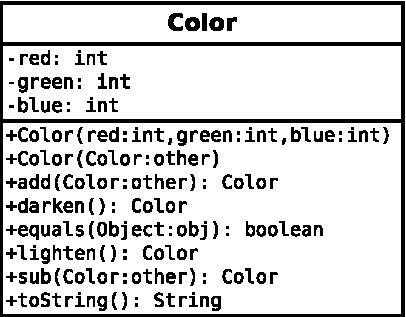
\includegraphics{CS1B/Color.pdf}
~~~~~
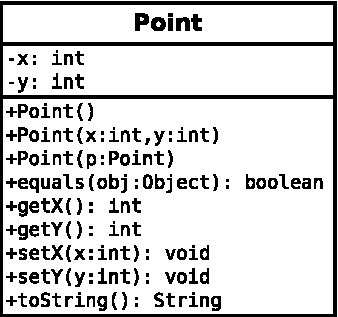
\includegraphics{CS1B/Point.pdf}
\end{center}

Classes generally include the following kinds of methods:
\begin{itemize}[itemsep=0pt]
\item \textbf{constructor} methods that initialize new objects
\item \textbf{accessor} methods (getters) that return attributes
\item \textbf{mutator} methods (setters) that modify attributes
\item \textbf{object} methods such as \java{equals} and \java{toString}
%\item \textbf{utility} methods which are generally static
\end{itemize}


\quest{15 min}


\Q Identify the constructors for the \java{Color} class. What is the difference between them? What arguments do they take? What do these methods return?

\begin{answer}
\end{answer}


\Q Identify an accessor method in the \java{Point} class. 
\begin{enumerate}[itemsep=0pt]
\item Which instance variable does it get?
\item What arguments does the method take?
\item What does the method return?
\end{enumerate}


\Q Identify a mutator method in the \java{Point} class.
\begin{enumerate}[itemsep=0pt]
\item Which instance variable does it set?
\item What arguments does the method take?
\item What does the method return?
\end{enumerate}


\begin{center}
\textit{For the remaining questions, you will design a class that represents an individual's credit card.}
\bigskip\par
% https://www.bankofamerica.com/credit-cards/
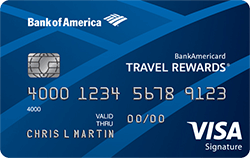
\includegraphics{CS1B/credit-card.png}
\end{center}


\Q List two or more attributes that would be necessary for this \java{CreditCard} class. For each attribute, indicate what data type would be most appropriate.

\begin{enumerate}
\item 
\item 
\end{enumerate}


\Q When constructing (or updating) a \java{CreditCard} object, what values would you need to check? What are the valid ranges of values for each attribute?

\begin{enumerate}
\item 
\item 
\end{enumerate}


\Q List two accessor methods would be appropriate for the \java{CreditCard} class.
Include arguments and return values, using the same format as a UML diagram.

\begin{enumerate}
\item 
\item 
\end{enumerate}


\Q List two mutator methods would be appropriate for the \java{CreditCard} class.
Include arguments and return values, using the same format as a UML diagram.

\begin{enumerate}
\item 
\item 
\end{enumerate}
